
\documentclass[11pt,a4paper]{article}
\usepackage[margin=1.7cm]{geometry}
\usepackage{amsmath,amssymb}
\usepackage{tikz}
\usepackage{xcolor}
\usepackage{parskip}
\usepackage[T1]{fontenc}
\usepackage[utf8]{inputenc}
\usepackage[dutch]{babel}
\usepackage{newtxtext,newtxmath}
\usetikzlibrary{arrows.meta,calc,positioning,decorations.pathmorphing}

\setlength{\parskip}{0.55em}
\setlength{\parindent}{0pt}

\newcommand{\uncertain}[1]{\textit{\textcolor{gray}{#1}}}

\newcommand{\atomcore}[1]{
\begin{tikzpicture}[scale=0.9]
    \fill[red!70] (0,0) circle (0.55);
    \draw[green!60!black, line width=2pt] (0,0) circle (0.75);
    #1
\end{tikzpicture}
}

\newcommand{\spiralpacket}[1]{
\draw[thick, #1] plot[smooth cycle, tension=0.8] coordinates
{(0,2.6) (1.4,2.1) (2.3,1.0) (2.4,-0.1) (1.7,-1.6) (0.2,-2.5) (-1.6,-2.2) (-2.5,-1.0) (-2.5,0.8) (-1.5,2.2)};
}

\title{Notebook 2012 --- Pagina's 43--47}
\author{}
\date{}

\begin{document}
\maketitle

\uncertain{Deze batch reconstrueert pagina's 43 t/m 47. Een aantal symbolen en woorden zijn licht onzeker door het handschrift en het scancontrast; zulke passages zijn zo letterlijk mogelijk weergegeven met minimale normalisatie.}

\clearpage
\section*{Pagina 43}

\begin{minipage}[t]{0.56\textwidth}
\subsection*{Linkerhelft}
\begin{align*}
\alpha_g &= \frac{G m_e^2}{\hbar c}
           = \left(l_p \omega_e\right)^2
\\[0.4em]
\left(\frac{m_e}{m_{\text{planck}}}\right)^2
&= 1{,}7518 \cdot 10^{-45}
\\[0.4em]
l_p &= \lambda_e \, \frac{\sqrt{\alpha_g}}{2\pi}
\\[0.4em]
\alpha_g &= \left(l_p \omega_e\right)^2 = l_p^2 \omega_e^2
\\[0.4em]
\alpha_g &= l_p^2 \frac{k_e}{m_e}
\approx l_p^2 \frac{F_{\max}}{a_0\,m_e}
\end{align*}

\uncertain{Rode notitie rechts: waarschijnlijk een analogie van de vorm
$\alpha = \left(\frac{q}{q_p}\right)^2$. De laatste term bevat een doorgestreepte correctie.}
\end{minipage}
\hfill
\begin{minipage}[t]{0.38\textwidth}
\subsection*{Rechterhelft}
\textbf{Minkowski Ruimte}

\medskip
\uncertain{Deze bladzijde is verder grotendeels leeg en bevat alleen de titel ``Minkowski Ruimte''.}
\end{minipage}

\clearpage
\section*{Pagina 44}

\begin{minipage}[t]{0.48\textwidth}
\subsection*{Linkerhelft}
\begin{flushleft}
Foton heeft ook een lading\\
en net zoals overal\\
zelfde lading stoot elkaar af.
\end{flushleft}

\begin{flushleft}
Maar hoe kon de foton\\
dan recht door ogen?
\end{flushleft}

\begin{flushleft}
De oneindige constructieve\\
golf interferentie
\end{flushleft}

\begin{flushleft}
Hoe kan dat?\\
de gulden snede en drie\\
dimensies
\end{flushleft}

\uncertain{Enkele woorden in de tweede en derde regel zijn licht onzeker; de strekking is wel duidelijk.}
\end{minipage}
\hfill
\begin{minipage}[t]{0.48\textwidth}
\subsection*{Rechterhelft}
{\color{red!75!black}\Large Wat is een Lading?}

\medskip

{\color{red!75!black}
een lading is een golf in tijdruimte\\
die golf is een rond draaiende lijn.
}

\medskip

\begin{center}
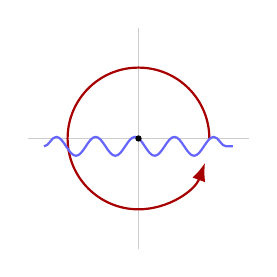
\begin{tikzpicture}[scale=1.0,>=Latex]
    \draw[gray!40] (-1.4,0) -- (1.4,0);
    \draw[gray!40] (0,-1.4) -- (0,1.4);
    \draw[red!65!black, thick, ->] (0.9,0) arc[start angle=0,end angle=340,radius=0.9];
    \draw[blue!60, thick, decorate, decoration={snake, amplitude=1.2mm, segment length=5mm}] (-1.2,-0.1) -- (1.2,-0.1);
    \fill[black] (0,0) circle (0.04);
\end{tikzpicture}
\end{center}

\uncertain{In het midden staat een zeer klein schetsje van een draaiende kring/golf.}
\end{minipage}

\clearpage
\section*{Pagina 45}

\begin{minipage}[t]{0.48\textwidth}
\subsection*{Linkerhelft}
\textbf{Boven aanzicht}

\[
v = \omega R_c
\]

\begin{center}
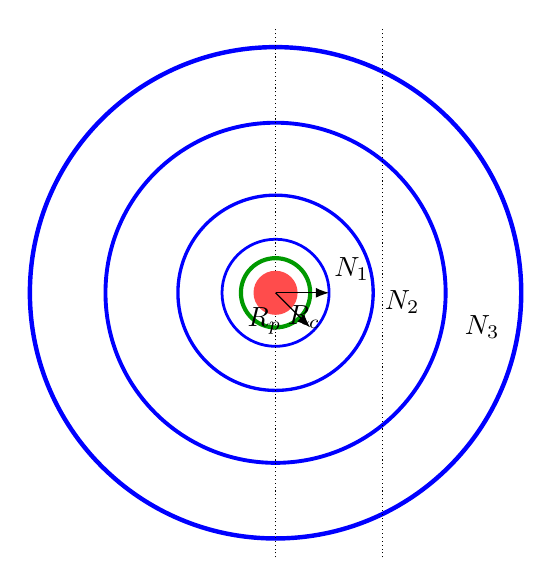
\begin{tikzpicture}[scale=0.8,>=Latex]
    \draw[blue, line width=1.6pt] (0,0) circle (3.9);
    \draw[blue, line width=1.4pt] (0,0) circle (2.7);
    \draw[blue, line width=1.2pt] (0,0) circle (1.55);
    \draw[blue, line width=1.0pt] (0,0) circle (0.85);
    \draw[densely dotted] (0,-4.2) -- (0,4.2);
    \draw[densely dotted] (1.7,-4.2) -- (1.7,4.2);
    \fill[red!70] (0,0) circle (0.35);
    \draw[green!60!black, line width=1.5pt] (0,0) circle (0.55);
    \draw[->] (0,0) -- (0.85,0);
    \node[below] at (0.45,-0.05) {$R_c$};
    \draw[->] (0,0) -- (0.55,-0.55);
    \node[left] at (0.25,-0.45) {$R_p$};
    \node[right] at (0.78,0.38) {$N_1$};
    \node[right] at (1.58,-0.15) {$N_2$};
    \node[right] at (2.85,-0.55) {$N_3$};
\end{tikzpicture}
\end{center}

grondstaat is een vaste vorm\\
en de kern van de\\
vrije vortex

\end{minipage}
\hfill
\begin{minipage}[t]{0.48\textwidth}
\subsection*{Rechterhelft}
\textbf{doorsnede van de torus}

\begin{center}
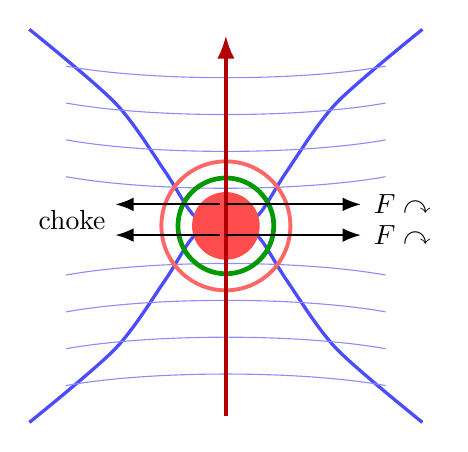
\begin{tikzpicture}[scale=0.78,>=Latex]
    % hourglass / throat
    \draw[blue!70, line width=1.2pt]
        plot[smooth] coordinates {(-3.2,3.2) (-1.8,2.0) (-1.0,0.9) (-0.55,0.2) (-0.2,0.0)};
    \draw[blue!70, line width=1.2pt]
        plot[smooth] coordinates {(3.2,3.2) (1.8,2.0) (1.0,0.9) (0.55,0.2) (0.2,0.0)};
    \draw[blue!70, line width=1.2pt]
        plot[smooth] coordinates {(-3.2,-3.2) (-1.8,-2.0) (-1.0,-0.9) (-0.55,-0.2) (-0.2,0.0)};
    \draw[blue!70, line width=1.2pt]
        plot[smooth] coordinates {(3.2,-3.2) (1.8,-2.0) (1.0,-0.9) (0.55,-0.2) (0.2,0.0)};
    % internal curved lines
    \foreach \y in {0.8,1.4,2.0,2.6} {
       \draw[blue!45] (-2.6,\y) .. controls (-1.2,\y-0.25) and (1.2,\y-0.25) .. (2.6,\y);
       \draw[blue!45] (-2.6,-\y) .. controls (-1.2,-\y+0.25) and (1.2,-\y+0.25) .. (2.6,-\y);
    }
    % central atom
    \fill[red!70] (0,0) circle (0.55);
    \draw[green!60!black, line width=1.7pt] (0,0) circle (0.78);
    \draw[red!60, line width=1.4pt] (0,0) circle (1.05);
    % axes/arrows
    \draw[red!70!black, very thick, ->] (0,-3.1) -- (0,3.1);
    \draw[black, thick, ->] (0.0,0.35) -- (2.2,0.35);
    \draw[black, thick, ->] (0.0,-0.15) -- (2.2,-0.15);
    \draw[black, thick, ->] (-0.1,0.35) -- (-1.8,0.35);
    \draw[black, thick, ->] (-0.1,-0.15) -- (-1.8,-0.15);
    \node[right] at (2.25,0.35) {$F \curvearrowright$};
    \node[right] at (2.25,-0.15) {$F \curvearrowright$};
    \node[left] at (-1.8,0.1) {choke};
\end{tikzpicture}
\end{center}

\uncertain{De scan toont een symmetrische torusdoorsnede met een vernauwing (``choke'') en radiale krachten.}
\end{minipage}

\clearpage
\section*{Pagina 46}

\begin{minipage}[t]{0.48\textwidth}
\subsection*{Linkerhelft}
\textbf{De vorm met eeuwige verdubbeling}

\[
\begin{array}{c|ccccccccccc}
n & 1 & 2 & 4 & 8 & 16 & 32 & 64 & 128 & 256 & 512 & 1024 \\
\hline
n \bmod 9 & 1 & 2 & 4 & 8 & 7 & 5 & 1 & 2 & 4 & 8 & 7
\end{array}
\]

\begin{center}
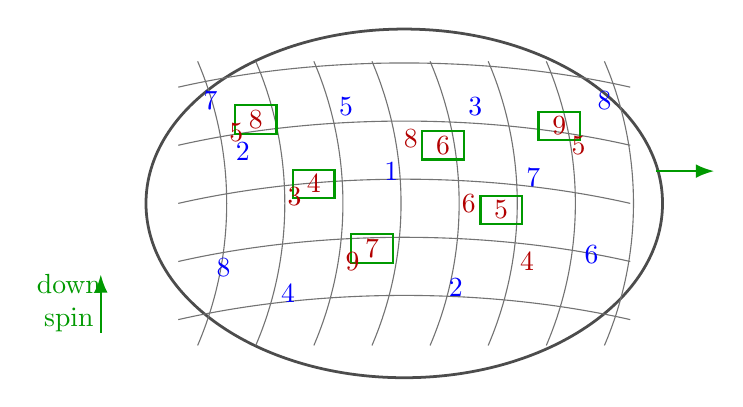
\begin{tikzpicture}[scale=0.82,>=Latex]
    % torus-like oval
    \draw[black!70, line width=1pt] (0,0) ellipse (4.0 and 2.7);
    % grid-ish curves
    \foreach \x in {-3.2,-2.3,-1.4,-0.5,0.4,1.3,2.2,3.1}{
      \draw[black!55] (\x,-2.2) .. controls (\x+0.6,-0.8) and (\x+0.6,0.8) .. (\x,2.2);
    }
    \foreach \y in {-1.8,-0.9,0,0.9,1.8}{
      \draw[black!55] (-3.5,\y) .. controls (-1.3,\y+0.5) and (1.3,\y+0.5) .. (3.5,\y);
    }
    % a few highlighted number boxes
    \foreach \cx/\cy/\val in {-2.3/1.3/8, -1.4/0.3/4, -0.5/-0.7/7, 0.6/0.9/6, 1.5/-0.1/5, 2.4/1.2/9}{
      \draw[green!60!black, thick] (\cx-0.32,\cy-0.22) rectangle (\cx+0.32,\cy+0.22);
      \node[red!70!black] at (\cx,\cy) {\val};
    }
    % blue and red digits scattered
    \foreach \cx/\cy/\val in {-3/1.6/7,-2.5/0.8/2,-2.8/-1.0/8,-1.8/-1.4/4,-0.9/1.5/5,-0.2/0.5/1,0.8/-1.3/2,1.1/1.5/3,2.0/0.4/7,2.9/-0.8/6,3.1/1.6/8}{
      \node[blue] at (\cx,\cy) {\val};
    }
    \foreach \cx/\cy/\val in {-2.6/1.1/5,-1.7/0.1/3,-0.8/-0.9/9,0.1/1.0/8,1.0/0.0/6,1.9/-0.9/4,2.7/0.9/5}{
      \node[red!70!black] at (\cx,\cy) {\val};
    }
    % arrows
    \draw[green!60!black, thick, ->] (-4.7,-2.0) -- (-4.7,-1.1);
    \node[green!60!black, left, align=center] at (-4.55,-1.55) {down\\spin};
    \draw[green!60!black, thick, ->] (3.9,0.5) -- (4.8,0.5);
\end{tikzpicture}
\end{center}
\end{minipage}
\hfill
\begin{minipage}[t]{0.48\textwidth}
\subsection*{Rechterhelft}
\begin{center}
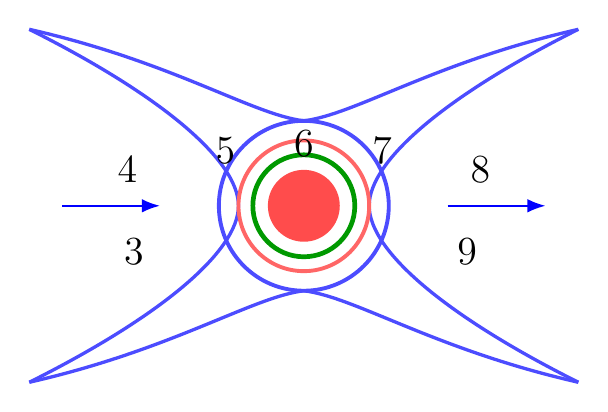
\begin{tikzpicture}[scale=0.83,>=Latex]
    % central torus cross
    \draw[blue!70, line width=1.4pt] (0,0) circle (1.3);
    \draw[blue!70, line width=1.2pt]
       (-4.2,2.7) .. controls (-2.0,2.2) and (-0.8,1.4) .. (0,1.3)
       .. controls (0.8,1.4) and (2.0,2.2) .. (4.2,2.7);
    \draw[blue!70, line width=1.2pt]
       (-4.2,-2.7) .. controls (-2.0,-2.2) and (-0.8,-1.4) .. (0,-1.3)
       .. controls (0.8,-1.4) and (2.0,-2.2) .. (4.2,-2.7);
    \draw[blue!70, line width=1.2pt]
       (-4.2,2.7) .. controls (-2.2,1.7) and (-1.0,0.7) .. (-1.0,0)
       .. controls (-1.0,-0.7) and (-2.2,-1.7) .. (-4.2,-2.7);
    \draw[blue!70, line width=1.2pt]
       (4.2,2.7) .. controls (2.2,1.7) and (1.0,0.7) .. (1.0,0)
       .. controls (1.0,-0.7) and (2.2,-1.7) .. (4.2,-2.7);
    % core
    \fill[red!70] (0,0) circle (0.55);
    \draw[green!60!black, line width=1.7pt] (0,0) circle (0.78);
    \draw[red!60, line width=1.4pt] (0,0) circle (1.0);
    % arrows and numbers
    \draw[blue, thick, ->] (-3.7,0.0) -- (-2.2,0.0);
    \draw[blue, thick, ->] (2.2,0.0) -- (3.7,0.0);
    \node at (-2.7,0.55) {\Large 4};
    \node at (-1.2,0.85) {\Large 5};
    \node at (0,0.95) {\Large 6};
    \node at (1.2,0.85) {\Large 7};
    \node at (2.7,0.55) {\Large 8};
    \node at (-2.6,-0.7) {\Large 3};
    \node at (2.5,-0.7) {\Large 9};
\end{tikzpicture}
\end{center}

\uncertain{De originele schets toont een getordeerde vorm met cijfers 1 t/m 9 en blauwe stroomrichtingen.}
\end{minipage}

\clearpage
\section*{Pagina 47}

\begin{minipage}[t]{0.48\textwidth}
\subsection*{Linkerhelft}
\[
\begin{array}{|ccc|ccc|}
\hline
5 & 7 & 8 & 4 & 2 & 1 \\
6 & 9 & 3 & 3 & 9 & 6 \\
1 & 2 & 4 & 8 & 7 & 5 \\
\hline
\end{array}
\qquad
\begin{array}{l}
578421 \\
124875
\end{array}
\]

\begin{center}
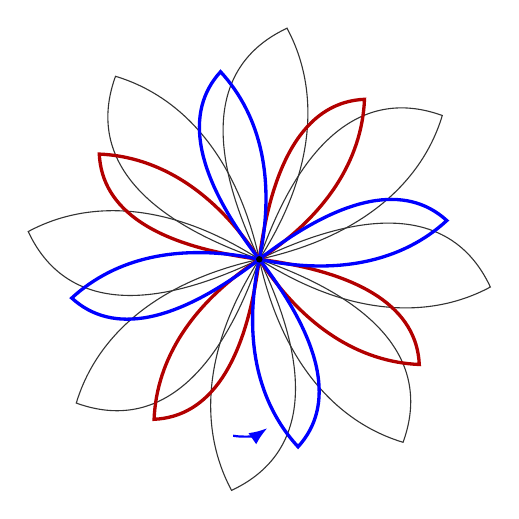
\begin{tikzpicture}[scale=0.83,>=Latex]
    % circular swirl petals
    \foreach \k in {0,45,90,135,180,225,270,315}{
      \begin{scope}[rotate=\k]
        \draw[black!80] (0,0) .. controls (1.6,0.35) and (2.5,1.2) .. (2.8,2.2)
                       .. controls (1.7,2.6) and (0.7,2.0) .. (0,0);
      \end{scope}
    }
    \foreach \k in {20,110,200,290}{
      \begin{scope}[rotate=\k]
        \draw[red!70!black, line width=1.2pt] (0,0) .. controls (1.2,0.28) and (2.0,0.9) .. (2.35,1.75)
                           .. controls (1.55,2.0) and (0.75,1.45) .. (0,0);
      \end{scope}
    }
    \foreach \k in {65,155,245,335}{
      \begin{scope}[rotate=\k]
        \draw[blue, line width=1.2pt] (0,0) .. controls (1.2,0.28) and (2.0,0.9) .. (2.35,1.75)
                           .. controls (1.55,2.0) and (0.75,1.45) .. (0,0);
      \end{scope}
    }
    \fill[black] (0,0) circle (0.05);
    \draw[blue, thick, ->] (-0.4,-2.7) arc[start angle=-100,end angle=-55,radius=0.7];
\end{tikzpicture}
\end{center}

\begin{flushright}
Vortex torus\\
Boven kant
\end{flushright}
\end{minipage}
\hfill
\begin{minipage}[t]{0.48\textwidth}
\subsection*{Rechterhelft}
\begin{center}
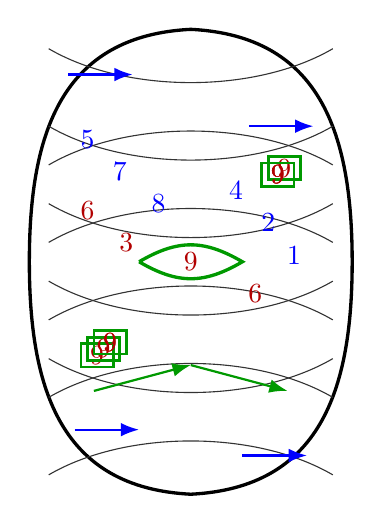
\begin{tikzpicture}[scale=0.82,>=Latex]
    % outer capsule
    \draw[black, line width=1.2pt] (0,3.6) .. controls (2.0,3.5) and (2.5,2.0) .. (2.5,0)
                                   .. controls (2.5,-2.0) and (2.0,-3.5) .. (0,-3.6)
                                   .. controls (-2.0,-3.5) and (-2.5,-2.0) .. (-2.5,0)
                                   .. controls (-2.5,2.0) and (-2.0,3.5) .. (0,3.6);
    % helical bands
    \foreach \s in {-2.4,-1.2,0,1.2,2.4}{
      \draw[black!80] (-2.2,\s+0.9) .. controls (-1.0,\s+0.2) and (1.0,\s+0.2) .. (2.2,\s+0.9);
      \draw[black!80] (-2.2,\s-0.9) .. controls (-1.0,\s-0.2) and (1.0,\s-0.2) .. (2.2,\s-0.9);
    }
    % center lozenge
    \draw[green!60!black, line width=1.2pt] (-0.8,0) .. controls (-0.2,0.35) and (0.2,0.35) .. (0.8,0)
                                             .. controls (0.2,-0.35) and (-0.2,-0.35) .. (-0.8,0);
    \node[red!70!black] at (0,0) {9};
    % small green cells
    \foreach \x/\y in {-1.45,1.35, -1.35,-1.25, 1.45,1.35, 1.35,-1.25} {
        \draw[green!60!black, line width=1.0pt] (\x-0.25,\y-0.18) rectangle (\x+0.25,\y+0.18);
        \node[red!70!black] at (\x,\y) {9};
    }
    % arrows
    \draw[blue, thick, ->] (-1.9,2.9) -- (-0.9,2.9);
    \draw[blue, thick, ->] (0.9,2.1) -- (1.9,2.1);
    \draw[blue, thick, ->] (-1.8,-2.6) -- (-0.8,-2.6);
    \draw[blue, thick, ->] (0.8,-3.0) -- (1.8,-3.0);
    \draw[green!60!black, thick, ->] (-1.5,-2.0) -- (0.0,-1.6);
    \draw[green!60!black, thick, ->] (0.0,-1.6) -- (1.5,-2.0);
    % a few digits
    \node[blue] at (-1.6,1.9) {5};
    \node[blue] at (-1.1,1.4) {7};
    \node[blue] at (-0.5,0.9) {8};
    \node[blue] at (0.7,1.1) {4};
    \node[blue] at (1.2,0.6) {2};
    \node[blue] at (1.6,0.1) {1};
    \node[red!70!black] at (-1.6,0.8) {6};
    \node[red!70!black] at (-1.0,0.3) {3};
    \node[red!70!black] at (1.0,-0.5) {6};
\end{tikzpicture}
\end{center}

\begin{flushright}
Vortex torus\\
Zijaanzicht
\end{flushright}
\end{minipage}

\end{document}
